% ============================================================
% Chapter 1: Descriptive Statistics
% ============================================================
\chapter{Descriptive Statistics --- Summary and Visualization}
\label{ch:descriptive}

\begin{center}
\textit{``You can't improve what you don't measure.''} --- Lord Kelvin
\end{center}

% ------------------------------------------------------------
\section{Motivating Example}
% ------------------------------------------------------------

A company has the monthly salaries (in euros) of its 20 employees:
\[
1800,\; 1950,\; 2100,\; 2100,\; 2200,\; 2300,\; 2350,\; 2400,\; 2500,\; 2600,
\]
\[
2650,\; 2700,\; 2800,\; 2900,\; 3100,\; 3200,\; 3500,\; 3800,\; 4500,\; 8000.
\]
Natural questions: What is the ``typical'' salary? How spread out are the salaries? Are there outliers? To answer these, we need to \emph{summarize} and \emph{visualize} the data.

% ------------------------------------------------------------
\section{Population, Sample, Variables}
% ------------------------------------------------------------

\begin{definition}[Population and Sample]
\index{population}\index{sample}
The \textbf{population} is the complete set of individuals under study. A \textbf{sample} of size $n$ is a subset $(x_1,\ldots,x_n)$ from the population.
\end{definition}

\begin{definition}[Types of Variables]
\index{variable!qualitative}\index{variable!quantitative}
\begin{itemize}
\item \textbf{Qualitative} (categorical): values in a finite set of categories.
  \begin{itemize}
  \item \emph{Nominal}: no natural ordering (color, sex).
  \item \emph{Ordinal}: natural ordering (grade: fail $<$ pass $<$ good $<$ excellent).
  \end{itemize}
\item \textbf{Quantitative}: numerical values.
  \begin{itemize}
  \item \emph{Discrete}: countable set ($\N$, number of children).
  \item \emph{Continuous}: values in an interval of $\R$ (height, weight).
  \end{itemize}
\end{itemize}
\end{definition}

% ------------------------------------------------------------
\section{Measures of Central Tendency}
% ------------------------------------------------------------

\begin{definition}[Arithmetic Mean]
\index{mean}
For a sample $(x_1,\ldots,x_n)$, the \textbf{mean} is:
\[
\bar{x} = \frac{1}{n}\sum_{i=1}^{n} x_i.
\]
\end{definition}

\begin{definition}[Median]
\index{median}
The \textbf{median} $\mathrm{Me}$ is the value that splits the ordered sample into two equal halves. If $x_{(1)}\leq x_{(2)}\leq\cdots\leq x_{(n)}$ denotes the order statistics:
\[
\mathrm{Me} = \begin{cases}
x_{((n+1)/2)} & \text{if } n \text{ is odd,}\\
\frac{1}{2}\left(x_{(n/2)}+x_{(n/2+1)}\right) & \text{if } n \text{ is even.}
\end{cases}
\]
\end{definition}

\begin{definition}[Mode]
\index{mode}
The \textbf{mode} is the most frequent value in the sample.
\end{definition}

\begin{intuition}
The mean is sensitive to extreme values; the median is \textbf{robust}. In the salary example, $\bar{x}=3007.50$~EUR is pulled upward by the 8000~EUR salary, while $\mathrm{Me}=2625$~EUR better reflects the ``typical'' salary.
\end{intuition}

% ------------------------------------------------------------
\section{Measures of Spread}
% ------------------------------------------------------------

\begin{definition}[Variance and Standard Deviation]
\index{variance}\index{standard deviation}
The \textbf{sample variance} (corrected) and \textbf{standard deviation} are:
\[
s^2 = \frac{1}{n-1}\sum_{i=1}^{n}(x_i-\bar{x})^2, \qquad s = \sqrt{s^2}.
\]
The uncorrected version uses $n$ in the denominator. The factor $n-1$ (Bessel's correction) ensures $s^2$ is an unbiased estimator of the population variance (cf.\ Chapter~\ref{ch:properties}).
\end{definition}

\begin{definition}[Range and Interquartile Range]
\index{range}\index{interquartile range}
\begin{align}
\text{Range} &= x_{(n)} - x_{(1)}, \\
\text{IQR} &= Q_3 - Q_1,
\end{align}
where $Q_1$ and $Q_3$ are the first and third quartiles.
\end{definition}

\begin{definition}[Coefficient of Variation]
\index{coefficient of variation}
$\mathrm{CV} = s/\bar{x}$ (for $\bar{x}\neq 0$). Allows comparison of spread across variables with different units.
\end{definition}

% ------------------------------------------------------------
\section{Shape Measures}
% ------------------------------------------------------------

\begin{definition}[Skewness]
\index{skewness}
\[
\gamma_1 = \frac{1}{n}\sum_{i=1}^n\left(\frac{x_i-\bar{x}}{s}\right)^3.
\]
$\gamma_1>0$: right-skewed. $\gamma_1<0$: left-skewed. $\gamma_1=0$: symmetric.
\end{definition}

\begin{definition}[Kurtosis]
\index{kurtosis}
\[
\gamma_2 = \frac{1}{n}\sum_{i=1}^n\left(\frac{x_i-\bar{x}}{s}\right)^4 - 3.
\]
$\gamma_2=0$ for a normal distribution. $\gamma_2>0$: heavy tails (leptokurtic). $\gamma_2<0$: light tails (platykurtic).
\end{definition}

% ------------------------------------------------------------
\section{Graphical Representations}
% ------------------------------------------------------------

\subsection{Histogram}
\index{histogram}

\begin{center}
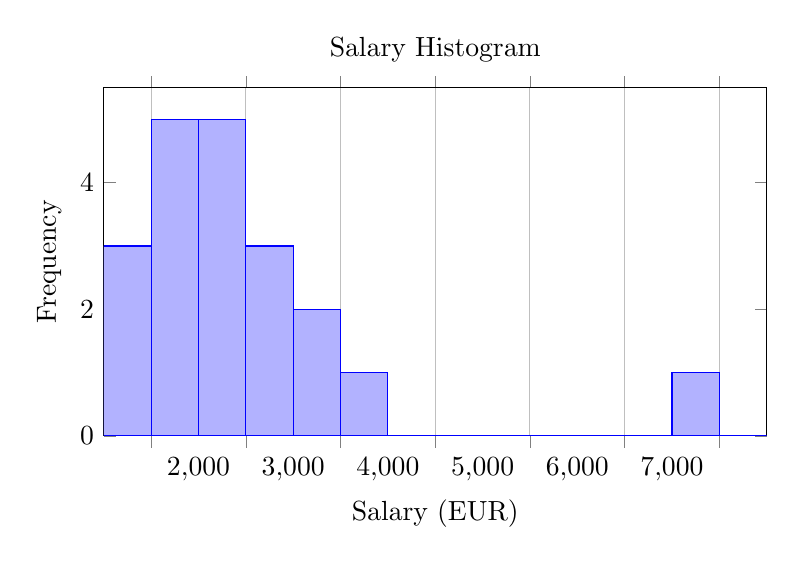
\begin{tikzpicture}
\begin{axis}[
    ybar interval,
    width=10cm, height=6cm,
    xlabel={Salary (EUR)},
    ylabel={Frequency},
    xmin=1500, xmax=8500,
    ymin=0,
    xtick={2000,3000,4000,5000,6000,7000,8000},
    title={Salary Histogram}
]
\addplot coordinates {
    (1500,3) (2000,5) (2500,5) (3000,3) (3500,2) (4000,1) (4500,0) (5000,0) (5500,0) (6000,0) (6500,0) (7000,0) (7500,1) (8000,0) (8500,0)
};
\end{axis}
\end{tikzpicture}
\end{center}

\subsection{Boxplot}
\index{boxplot}

\begin{center}
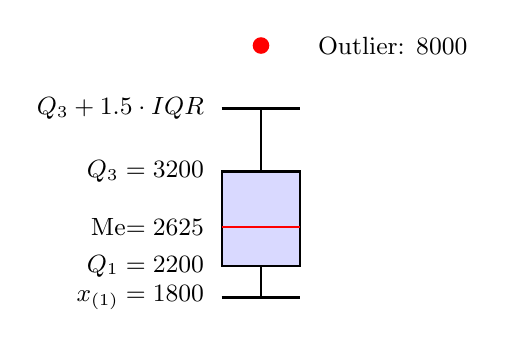
\begin{tikzpicture}
  \draw[thick] (2,0) -- (2,0.4);
  \draw[thick] (1.5,0) -- (2.5,0);
  \draw[thick,fill=blue!15] (1.5,0.4) rectangle (2.5,1.6);
  \draw[thick,red] (1.5,0.9) -- (2.5,0.9);
  \draw[thick] (2,1.6) -- (2,2.4);
  \draw[thick] (1.5,2.4) -- (2.5,2.4);
  \fill[red] (2,3.2) circle (3pt);
  \node[left] at (1.4,0) {\small $x_{(1)}=1800$};
  \node[left] at (1.4,0.4) {\small $Q_1=2200$};
  \node[left] at (1.4,0.9) {\small Me$=2625$};
  \node[left] at (1.4,1.6) {\small $Q_3=3200$};
  \node[left] at (1.4,2.4) {\small $Q_3+1.5\cdot\text{IQR}$};
  \node[right] at (2.6,3.2) {\small Outlier: $8000$};
\end{tikzpicture}
\end{center}

\subsection{Empirical Distribution Function}
\index{empirical distribution function}

\begin{definition}
The \textbf{empirical distribution function} (ECDF) is:
\[
\hat{F}_n(x) = \frac{1}{n}\sum_{i=1}^n \mathbf{1}_{x_i \leq x}.
\]
It is a step function that approximates the true CDF $F$ (Glivenko--Cantelli theorem, cf.\ Chapter~\ref{ch:model}).
\end{definition}

% ------------------------------------------------------------
\section{Bivariate Data}
% ------------------------------------------------------------

\begin{definition}[Covariance and Correlation]
\index{covariance}\index{correlation}
For paired data $(x_1,y_1),\ldots,(x_n,y_n)$:
\begin{align}
s_{xy} &= \frac{1}{n-1}\sum_{i=1}^n (x_i-\bar{x})(y_i-\bar{y}), \\
r_{xy} &= \frac{s_{xy}}{s_x\cdot s_y} \in [-1,1].
\end{align}
$r_{xy}$ measures the \emph{linear association} between $x$ and $y$.
\end{definition}

\begin{warning}
Correlation does not imply causation. Two variables can be strongly correlated without a causal link (confounding variable, coincidence).
\end{warning}

\begin{center}
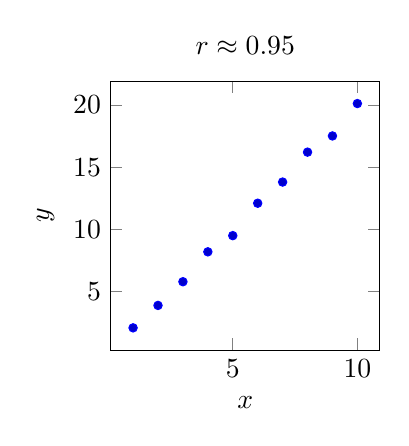
\begin{tikzpicture}
\begin{axis}[width=5cm, height=5cm, title={$r\approx 0.95$}, xlabel=$x$, ylabel=$y$, only marks, mark size=1.5pt]
\addplot coordinates {(1,2.1)(2,3.9)(3,5.8)(4,8.2)(5,9.5)(6,12.1)(7,13.8)(8,16.2)(9,17.5)(10,20.1)};
\end{axis}
\end{tikzpicture}
\hspace{1cm}
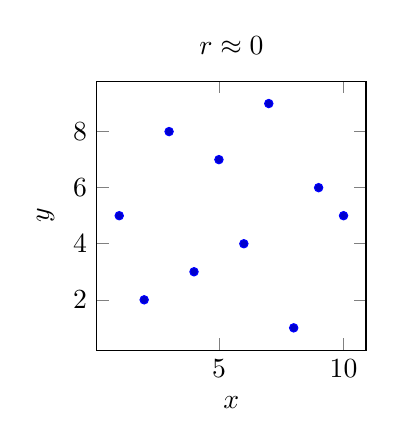
\begin{tikzpicture}
\begin{axis}[width=5cm, height=5cm, title={$r\approx 0$}, xlabel=$x$, ylabel=$y$, only marks, mark size=1.5pt]
\addplot coordinates {(1,5)(2,2)(3,8)(4,3)(5,7)(6,4)(7,9)(8,1)(9,6)(10,5)};
\end{axis}
\end{tikzpicture}
\hspace{1cm}
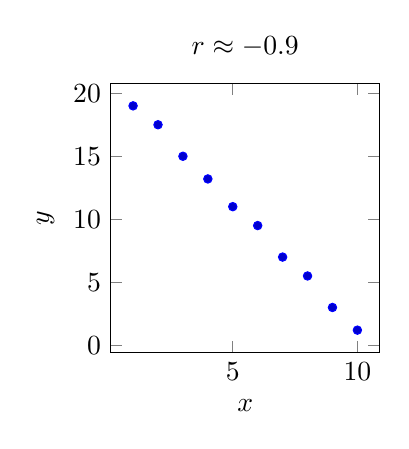
\begin{tikzpicture}
\begin{axis}[width=5cm, height=5cm, title={$r\approx -0.9$}, xlabel=$x$, ylabel=$y$, only marks, mark size=1.5pt]
\addplot coordinates {(1,19)(2,17.5)(3,15)(4,13.2)(5,11)(6,9.5)(7,7)(8,5.5)(9,3)(10,1.2)};
\end{axis}
\end{tikzpicture}
\end{center}

% ------------------------------------------------------------
\section{Python Implementation}
% ------------------------------------------------------------

\begin{python}
\begin{minted}{python}
import numpy as np
import pandas as pd
import matplotlib.pyplot as plt
from scipy import stats

salaries = np.array([1800, 1950, 2100, 2100, 2200, 2300, 2350, 2400,
                     2500, 2600, 2650, 2700, 2800, 2900, 3100, 3200,
                     3500, 3800, 4500, 8000])

print(f"Mean     : {np.mean(salaries):.2f}")
print(f"Median   : {np.median(salaries):.2f}")
print(f"Std dev  : {np.std(salaries, ddof=1):.2f}")
print(f"IQR      : {stats.iqr(salaries):.2f}")
print(f"Skewness : {stats.skew(salaries):.4f}")
print(f"Kurtosis : {stats.kurtosis(salaries):.4f}")

fig, axes = plt.subplots(1, 3, figsize=(14, 4))
axes[0].hist(salaries, bins=8, edgecolor='black', alpha=0.7)
axes[0].set_title("Histogram")
axes[1].boxplot(salaries, vert=True)
axes[1].set_title("Boxplot")
x_sorted = np.sort(salaries)
y_ecdf = np.arange(1, len(x_sorted)+1) / len(x_sorted)
axes[2].step(x_sorted, y_ecdf, where='post')
axes[2].set_title("ECDF")
plt.tight_layout()
plt.savefig("ch01_descriptive.pdf")
plt.show()
\end{minted}
\end{python}

% ------------------------------------------------------------
\section{Exercises}
% ------------------------------------------------------------

\begin{exercise}[$\star$ -- Basic calculations]
Temperatures (${}^\circ$C) over 10 days: $12, 14, 15, 13, 16, 18, 14, 15, 17, 16$. Compute mean, median, mode, variance, standard deviation, and IQR. Plot the histogram and boxplot.
\end{exercise}

\begin{exercise}[$\star$ -- Bivariate data]
Compute the correlation coefficient between midterm and final exam scores for 8 students and interpret.
\end{exercise}

\begin{exercise}[$\star\star$ -- Properties of the mean]
\begin{enumerate}
\item Show that $\sum_{i=1}^n (x_i - \bar{x}) = 0$.
\item Show that $\bar{x}$ minimizes $\sum_{i=1}^n (x_i - c)^2$ over $c\in\R$.
\item Deduce that $s^2 = \frac{1}{n-1}\left(\sum x_i^2 - n\bar{x}^2\right)$.
\end{enumerate}
\end{exercise}

\begin{exercise}[$\star\star$ -- Empirical Chebyshev inequality]
Show that for any $k>0$, the proportion of observations with $|x_i-\bar{x}|>ks$ is at most $1/k^2$.
\end{exercise}

\begin{exercise}[$\star\star\star$ -- Project: Exploratory data analysis]
Download a real dataset. Produce a complete report: descriptive statistics, visualizations, outlier identification, distribution shape commentary.
\end{exercise}

% ------------------------------------------------------------
\begin{keyformulas}
\begin{align*}
\bar{x} &= \frac{1}{n}\sum_{i=1}^n x_i &
s^2 &= \frac{1}{n-1}\sum_{i=1}^n(x_i-\bar{x})^2 \\
\mathrm{IQR} &= Q_3 - Q_1 &
r_{xy} &= \frac{s_{xy}}{s_x s_y} \\
\gamma_1 &= \frac{1}{n}\sum\left(\frac{x_i-\bar{x}}{s}\right)^3 &
\gamma_2 &= \frac{1}{n}\sum\left(\frac{x_i-\bar{x}}{s}\right)^4-3
\end{align*}
\end{keyformulas}
